% !TEX root = tracking.tex
\section{10D Quadrotor RRT Example \label{sec:results}}
\begin{figure*}
	\centering
	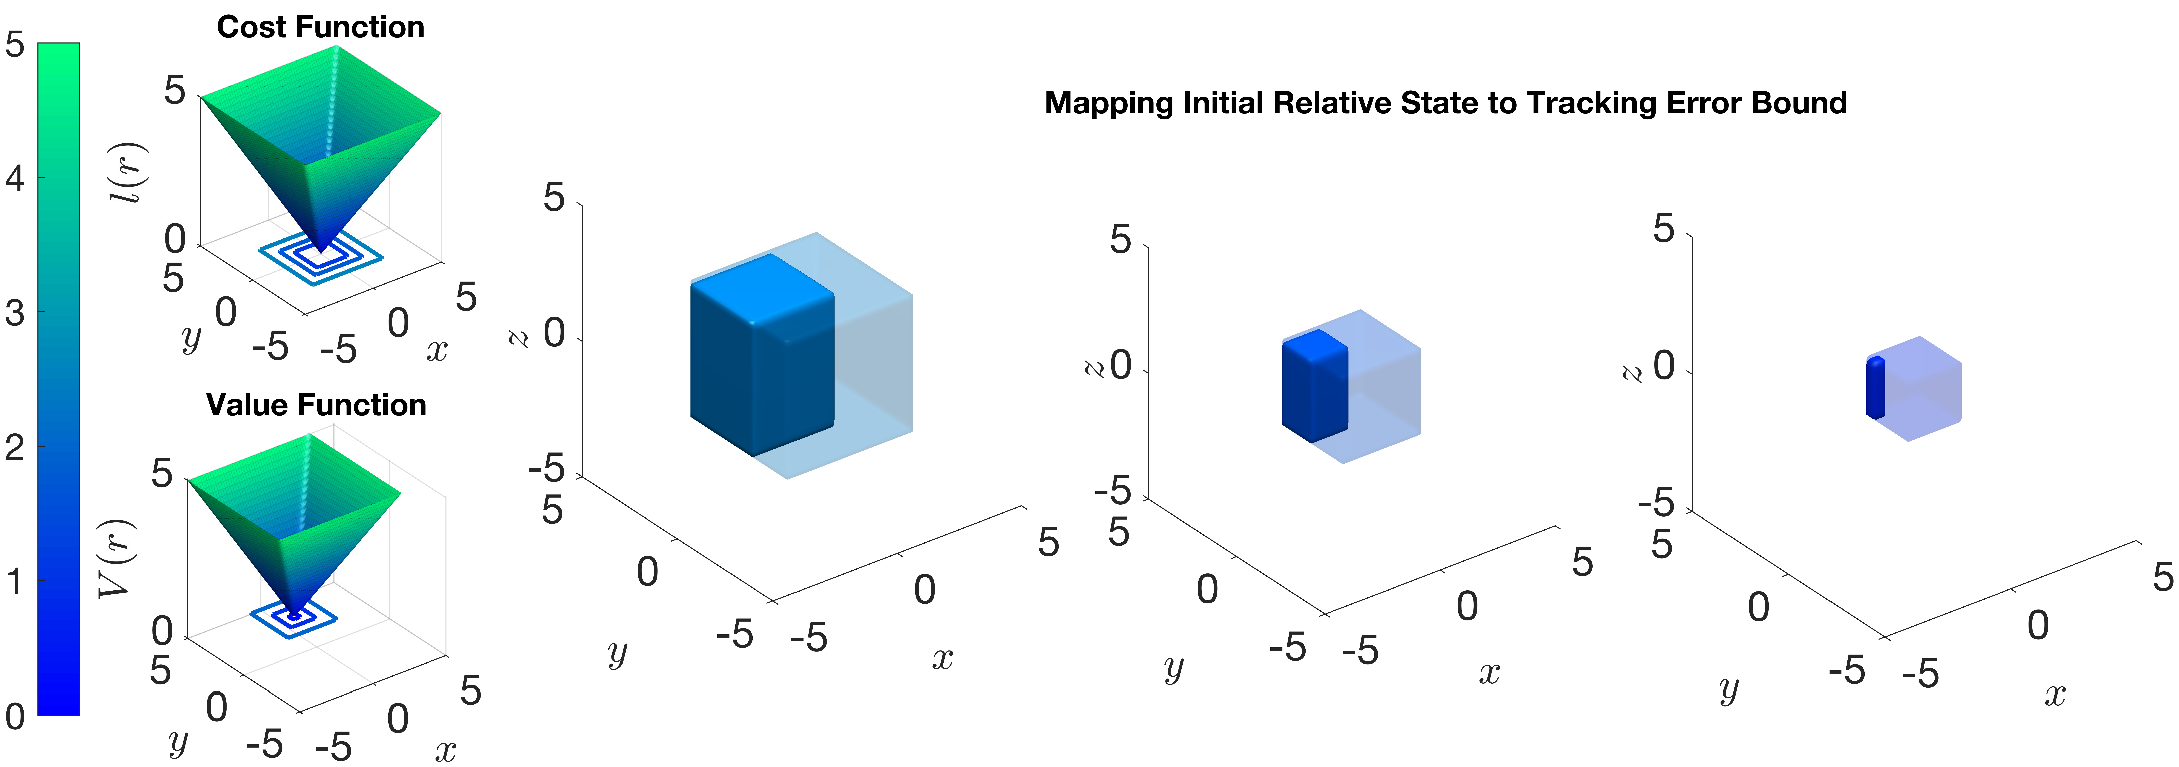
\includegraphics[width=0.7\textwidth]{fig/quad10D_example_cost}
	\caption{On the left are the cost and value functions over a 2D slice of the 10D relative state space, with contour lines showing three level sets of these functions. On the right are 3D projections of these level sets at the same slice $(v_{x},v_{y},v_{z})=[1, -1, 1]$ m/s, $(\theta_{x},\omega_{x},\theta_{y},\omega_{y})=0$. The solid boxes show initial relative states, and the transparent boxes show the corresponding tracking error bound. In practice we set the initial relative states to 0 to find the smallest invariant tracking error bound.}
	\label{fig:quad10D_example}
		\vspace{-.2in}
	\end{figure*} 
\begin{figure}
	\centering
	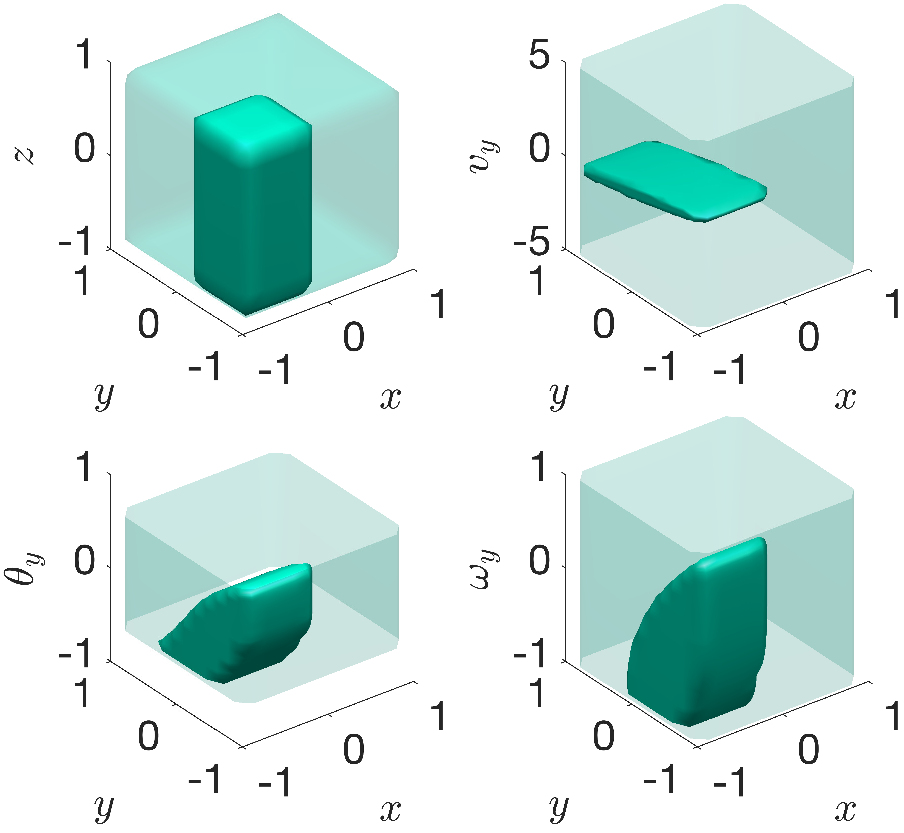
\includegraphics[width=0.25\textwidth]{fig/quad10D_slices}
	\caption{Various 3D slices of the 10D relative states (solid) and the corresponding tracking error bound (transparent)}
	\label{fig:quad10D_example_slices}
		\vspace{-.21in}
\end{figure} 
We demonstrate this framework with a 10D near-hover quadrotor developed in \cite{Bouffard12} tracking a 3D point source path generated by an RRT planner \cite{Kuffner2000},\cite{Kavraki1996}. First we perform the offline computations to acquire the tracking error bound and safety controller look-up tables. Next we set up the RRT to convert paths to simple 3D trajectories. Finally we implement the online framework to navigate the 10D system through a 3D environment with static obstacles.

\subsection{Precomputation of 10D-3D system}
First we define the 10D dynamics of the tracking quadrotor and the 3D dynamics of a holonomic vehicle:
\begin{equation}
\label{eq:Quad10D_dyn}
\begin{aligned}
\begin{array}{c}
\left[
\begin{array}{c}
\dot{x}\\
\dot{v_x}\\
\dot{\theta_x}\\
\dot\omega_x\\
\dot{y}\\
\dot{v_y}\\
\dot{\theta_y}\\
\dot\omega_y\\
\dot{z}\\
\dot{v_z}
\end{array}
\right]
=
\left[
\begin{array}{c}
v_x + d_x\\
g \tan \theta_x\\
-d_1 \theta_x + \omega_x\\
-d_0 \theta_x + n_0 a_x\\
v_y + d_y\\
g \tan \theta_y\\
-d_1 \theta_y + \omega_y\\
-d_0 \theta_y + n_0 a_y\\
v_z + d_z\\
k_T a_z - g
\end{array}
\right]
\left[
\begin{array}{c}
\dot{x}\\
\dot{y}\\
\dot{z}\\
\end{array}
\right] 
=
\left[
\begin{array}{c}
b_x\\
b_y\\
b_z \\
\end{array}
\right]
\end{array}\\
\end{aligned}
\end{equation}
where states $(x, y, z)$ denote the position, $(v_x, v_y, v_z)$ denote the velocity, $(\theta_x, \theta_y)$ denote the pitch and roll, and $(\omega_x, \omega_y)$ denote the pitch and roll rates. The controls of the 10D system are $(a_x, a_y, a_z)$, where $a_x$ and $a_y$ represent the desired pitch and roll angle, and $a_z$ represents the vertical thrust. The 3D system controls are $(b_x, b_y, b_z)$, and represent the velocity in each positional dimension. The disturbances in the 10D system $(d_x, d_y, d_z)$ are caused by wind, which acts on the velocity in each dimension. Note that the states of the 3D dynamics are a subset of the 10D state space; the matrix Q used in the online computation matches the position states of both systems. Next the relative dynamics between the two systems is defined using (\ref{eq:rdyn}):
\begin{equation}
\label{eq:Quad10DRel_dyn}
\begin{aligned}
\begin{array}{c}
\left[
\begin{array}{c}
\dot{x_r}\\
\dot{v_{x}}\\
\dot{\theta_{x}}\\
\dot\omega_{x}\\
\dot{y_r}\\
\dot{v_{y}}\\
\dot{\theta_{y}}\\
\dot\omega_{y}\\
\dot{z_r}\\
\dot{v_{z}}
\end{array}
\right]
=
\left[
\begin{array}{c}
v_x - b_x + d_x\\
g \tan \theta_x\\
-d_1 \theta_x + \omega_x\\
-d_0 \theta_x + n_0 a_x\\
v_y - b_y + d_y\\
g \tan \theta_y\\
-d_1 \theta_y + \omega_y\\
-d_0 \theta_y + n_0 a_y\\
v_z - b_z + d_z\\
k_T a_z - g
\end{array}
\right]
\end{array}\\
\end{aligned}
\end{equation}
The values for parameters $d_0,d_1,n_0,k_T,g$ used were: $d_0=10,d_1=8,n_0=10,k_T=0.91,g=9.81$. The 10D control bounds were $|a_x|,|a_y|\leq10$ degrees, $0\leq a_z\leq 1.5g$ m/s$^{2}$. The 3D control bounds were $|b_x|,|b_y|,|b_z|\leq0.5$ m/s. The disturbance bounds were $|d_x|,|d_y|,|d_z|\leq0.1$ m/s. 

Next we follow the setup in section \ref{sec:precomp} to create a cost function, which we then evaluate using HJ reachability until convergence to produce the invariant value function as in (\ref{eq:valfunc}). Historically this 10D nonlinear relative system would be intractable for HJ reachability analysis, but using new methods in \cite{Chen2016DecouplingExact, Chen2016DecouplingJournal} we can decompose this system into 3 subsystems (for each positional dimension). Doing this also requires decomposing the cost function; therefore we represent the cost function as a 1-norm instead of a 2-norm. This cost function as well as the resulting value function can be seen projected onto the $x,y$ dimensions in Fig. \ref{fig:quad10D_example}.

Fig. \ref{fig:quad10D_example} also shows 3D positional projections of the mapping between initial relative state to maximum potential relative distance over all time (i.e. tracking error bound). If the real system starts exactly at the origin in relative coordinates, its tracking error bound will be a box of $\underline\valfunc = 0.81$ m in each direction. Slices of the 3D set and corresponding tracking error bounds are also shown in Fig. \ref{fig:quad10D_example_slices}. We save the look-up tables of the value function (i.e. the tracking error function) and its spatial gradients (i.e. the safety controller function).

\subsection{Online Planning with RRT and Sensing}
Our precomputed value function can serve as a tracking error bound, and its gradients form a look-up table for the optimal tracking controller. These can be combined with any planning algorithm such as MPC, RRT, or neural-network-based planners in a modular way. 

To demonstrate the combination of fast planning and provably robust tracking, we used a simple multi-tree RRT planner implemented in MATLAB modified from \cite{Gavin2013}. We assigned a speed of $0.5$ m/s to the piecewise linear paths obtained from the RRT planner, so that the planning model is as given in \eqref{eq:Quad10D_dyn}. Besides planning a path to the goal, the quadrotor must also sense obstacles in the vicinity. For illustration, we chose a simple virtual sensor that reveals obstacles within a range of 2 m in the $x$, $y$, or $z$ directions.

Once an obstacle is sensed, the RRT planner replans while taking into account all obstacles that have been sensed so far. To ensure that the quadrotor does not collide with the obstacles despite error in tracking, planning is done with respect to augmented obstacles that are ``expanded'' from the sensed obstacles by $\underline\valfunc$ in the $x$, $y$, and $z$ directions.

On an unoptimized MATLAB implementation on a desktop computer with a Core i7-2600K CPU, each iteration took approximately $25$ ms on average. Most of this time is spent on planning: obtaining the tracking controller took approximately $5$ ms per iteration on average. The frequency of control was once every $100$ ms.

Fig. \ref{fig:sim} shows the simulation results. Four time snapshots are shown. The initial position is $(-12, 0, 0)$, and the goal position is $(12, 0, 0)$. The top left subplot shows the entire trajectory from beginning to end. In all plots, a magenta star represents the position of the planning model; its movement is based on the paths planned by RRT, and is modeled by a 3D holonomic vehicle with a maximum speed. The blue box around the magenta star represents the tracking error bound.
\begin{figure}
	\centering
	\begin{subfigure}[t]{0.49\columnwidth} \label{subfig:sim_4}
		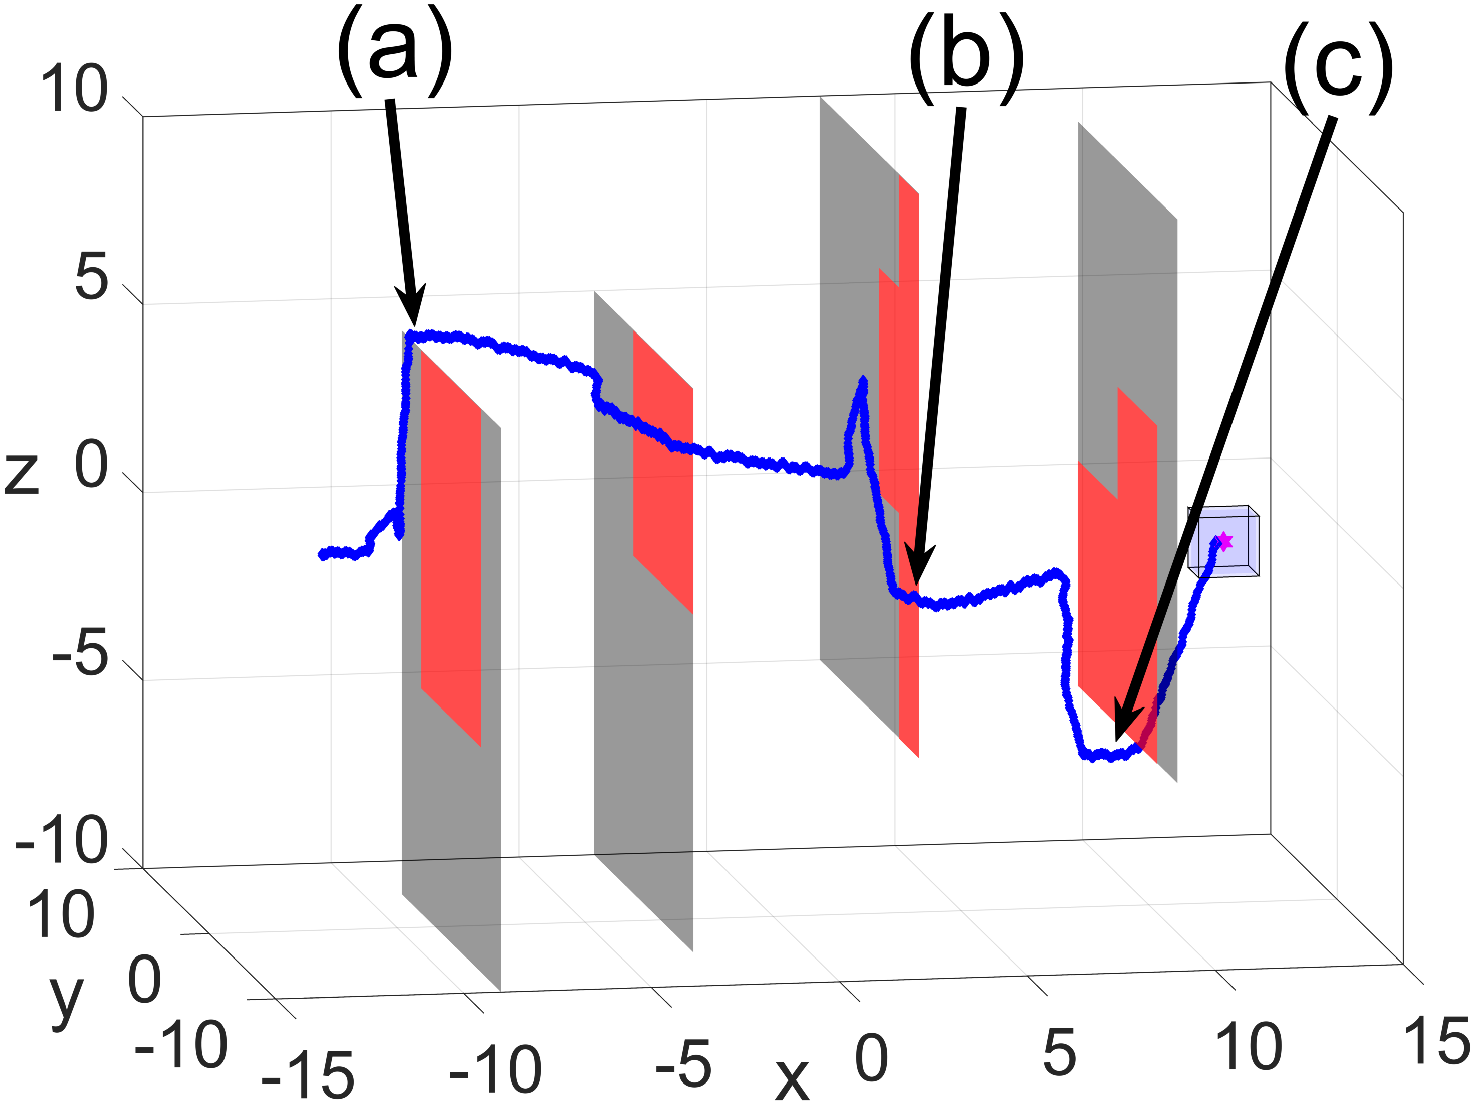
\includegraphics[width=\columnwidth]{fig/1173}
	\end{subfigure}  
	\begin{subfigure}[t]{0.49\columnwidth} \label{subfig:sim_1}
		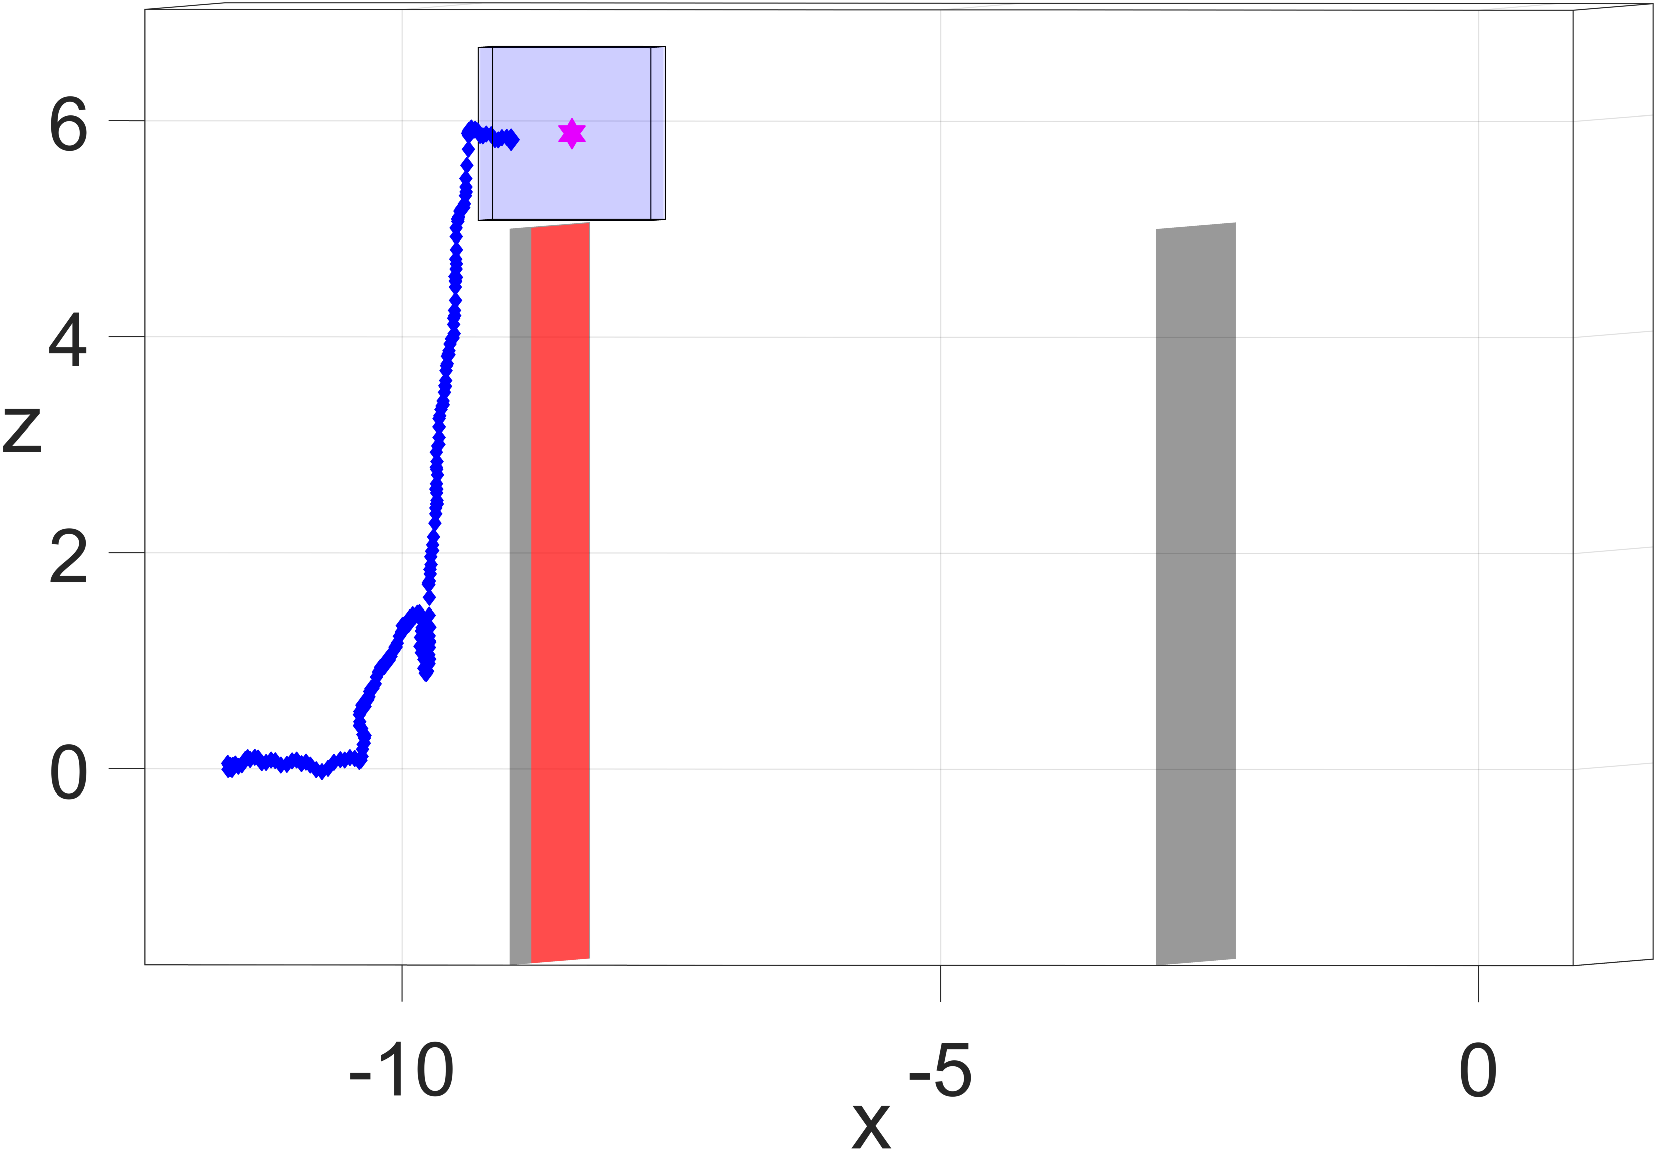
\includegraphics[width=\columnwidth]{fig/224}
		\caption{}
	\end{subfigure}
	
	\begin{subfigure}[t]{0.49\columnwidth} \label{subfig:sim_2}
		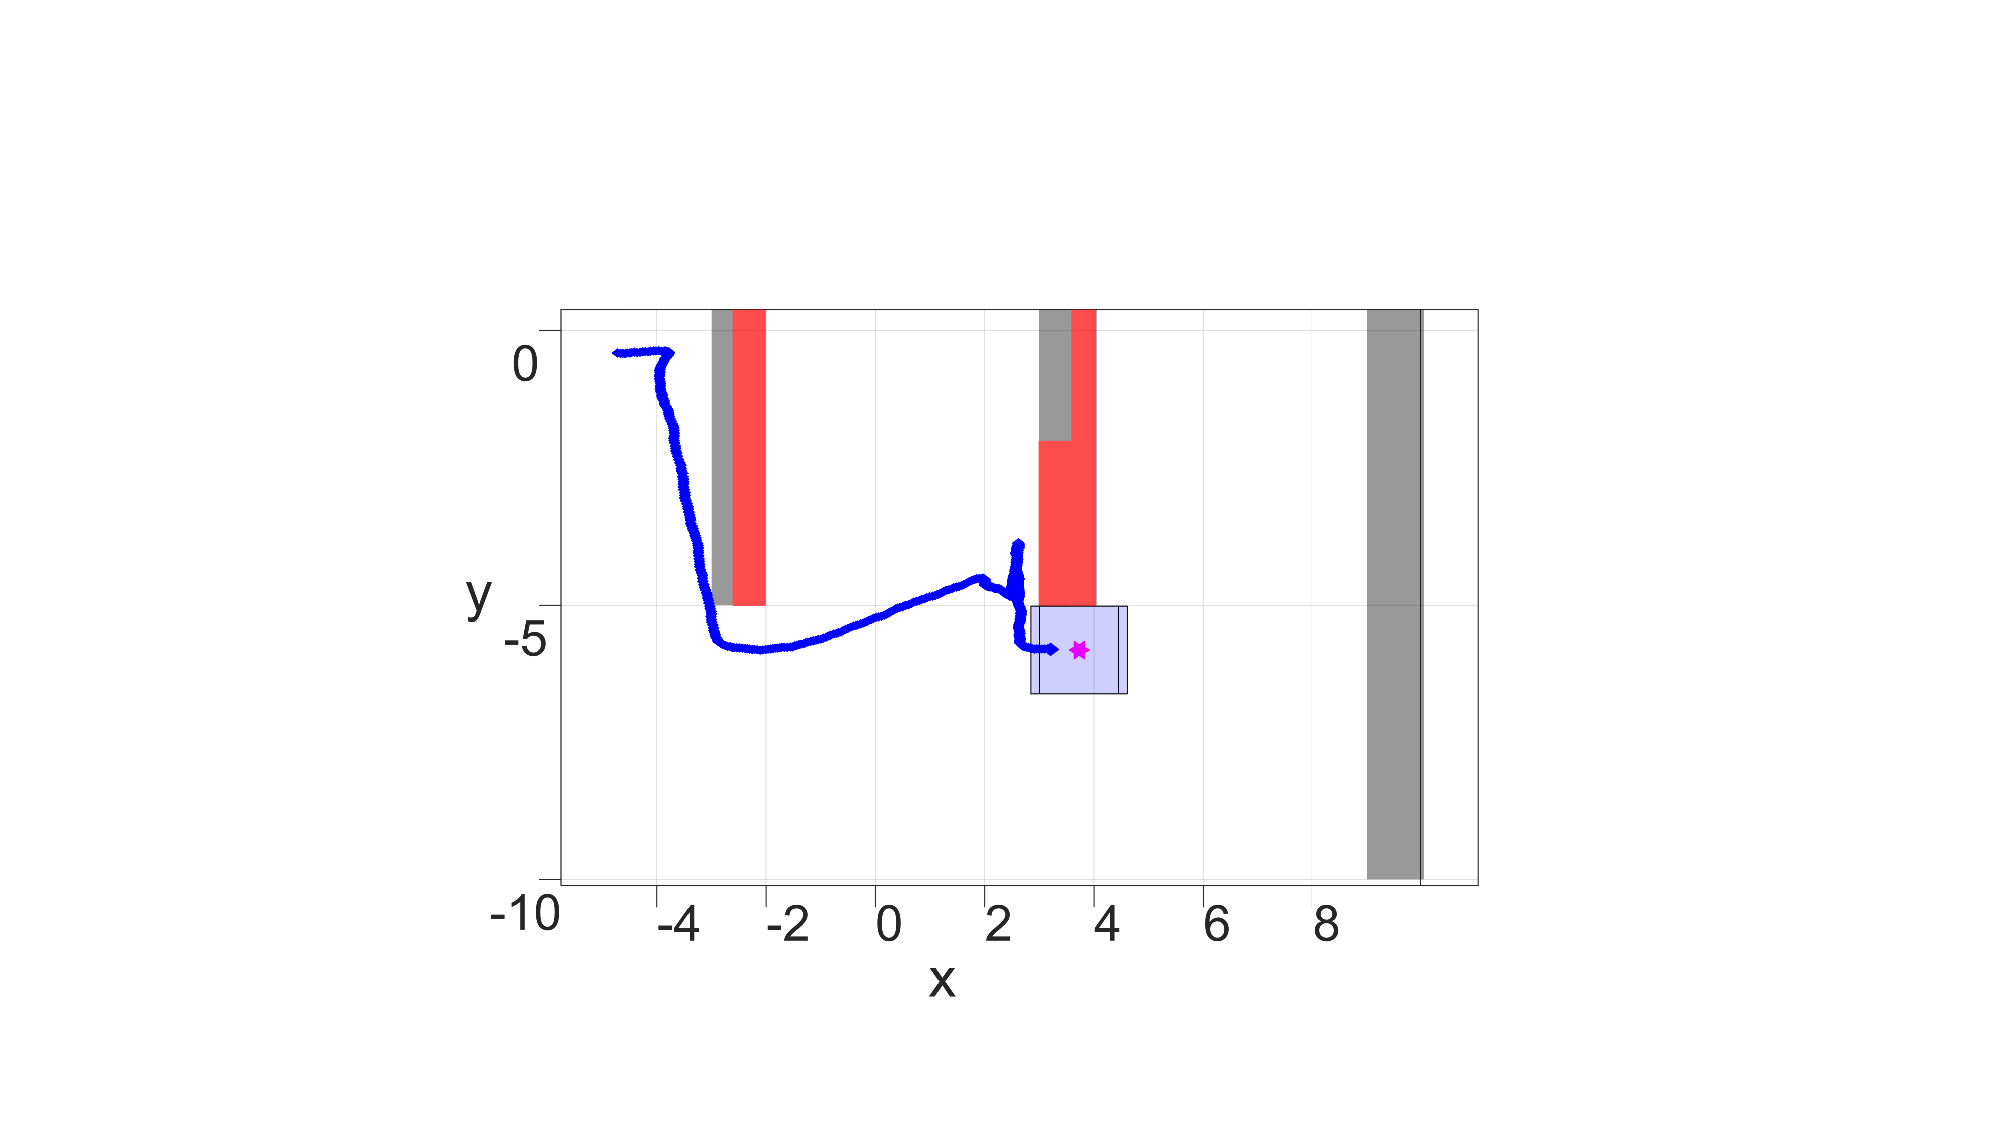
\includegraphics[width=\columnwidth]{fig/763}
		\caption{}
	\end{subfigure}  
	\begin{subfigure}[t]{0.49\columnwidth} \label{subfig:sim_3}
		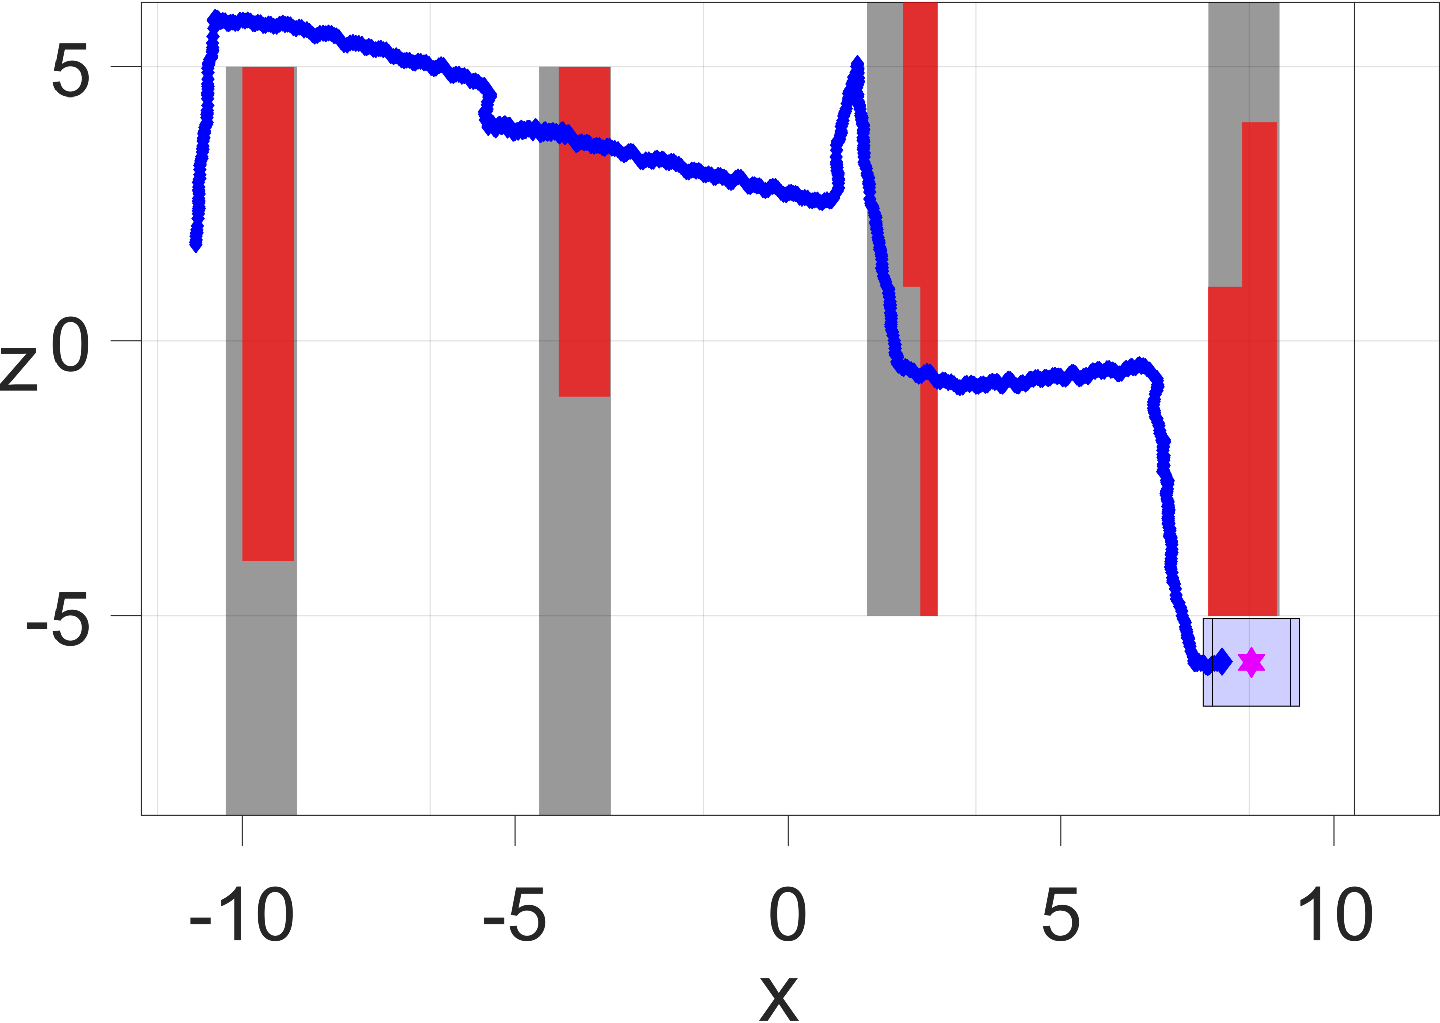
\includegraphics[width=\columnwidth]{fig/1042}
		\caption{}
	\end{subfigure}
	\vspace{-.1in}
	\caption{Numerical simulation. The tracking model trajectory is shown in blue, the planning model position in magenta, unseen obstacles in gray, and seen obstacles in red. The translucent blue box represents the tracking error bound. The top left subplot shows the entire trajectory; the other subplots zoom in on the positions marked in the top left subplot. The camera angle is also adjusted to illustrate our theoretical guarantees on tracking error and robustness in planning. A video of this simulation can be found at https://youtu.be/ZVvyeK-a62E \label{fig:sim}}
	\vspace{-.2in}
\end{figure}
The position of the tracking model is shown in blue. Throughout the simulation, the tracking model's position is always inside the tracking error, in agreement with Proposition \ref{prop:main}. In addition, the tracking error bound never intersects with the obstacles, a consequence of the RRT planner planning with respect to a set of augmented obstacles (not shown). In the latter two subplots, one can see that the quadrotor appears to be exploring the environment briefly before reaching the goal. In this paper, we did not employ any exploration algorithm; this exploration behavior is simply emerging from replanning using RRT whenever a new part (a $3$ m$^2$ portion) of an obstacle is sensed.